\documentclass[c]{beamer}

\usepackage{graphicx}
\usepackage{epsfig}
\usepackage{hyperref}
\usepackage{booktabs, caption}
\usepackage{anyfontsize}

% suppress navigation bar
\beamertemplatenavigationsymbolsempty

\mode<presentation>
{
  \usetheme{jd}
  \setbeamercovered{transparent}
  \setbeamertemplate{items}[circle]
}

% set fonts
\usepackage{fontspec}
\setsansfont{Changa One}
%\setmainfont{Fontin}
\setbeamerfont{frametitle}{size=\LARGE,series=\bfseries}

\usepackage{setspace}
\setstretch{3}
\parindent 0pt

% color definitions
\usepackage{color}
\definecolor{uipoppy}{RGB}{225, 64, 5}
\definecolor{uipaleblue}{RGB}{96,123,139}
\definecolor{uiblack}{RGB}{0, 0, 0}
\definecolor{uigreen}{RGB}{96, 147, 115}
\definecolor{uigreen_dark}{RGB}{31, 39, 42}
\definecolor{uigray}{RGB}{217, 217, 217}
\definecolor{uigray2}{RGB}{117, 117, 117}
\definecolor{uired}{RGB}{187, 114, 101}

\definecolor{blue1}{RGB}{41, 128, 185}
\definecolor{blue2}{RGB}{52, 152, 219}
\definecolor{blue3}{RGB}{44, 62, 80}
\definecolor{turquoise}{RGB}{22, 160, 133}
\definecolor{green1}{RGB}{39, 174, 96}

\definecolor{yellow1}{RGB}{241, 196, 15}
\definecolor{orange1}{RGB}{243, 156, 18}

% caption styling
\DeclareCaptionFont{uiblack}{\color{uiblack}}
\DeclareCaptionFont{uipoppy}{\color{uipoppy}}
\captionsetup{labelfont={uipoppy},textfont=uiblack}

% itemize style
\setbeamertemplate{itemize item}{\Huge\raise2.55pt\hbox{\donotcoloroutermaths\cred{$\blacktriangleright$}}}

% see the macros.tex file for definitions
% This program can be redistributed and/or modified under the terms
% of the GNU Public License, version 3.

% adds reference to bottom right of corner of a slide
\usepackage[absolute,overlay]{textpos} % text references in slide corners
\newcommand\textref[1]{%
  \begin{textblock*}{\paperwidth}(0pt,0.99\textheight)
  \raggedleft \tiny{\emph{#1}}\hspace{.5em}
  \end{textblock*}}

% for drawing circles around numbers
% ex. \circled{1} Add some text here.
\usepackage{tikz}
\usepackage{ifthen}
\usetikzlibrary{arrows}
\usetikzlibrary{matrix}
\usetikzlibrary{decorations,arrows}
\usetikzlibrary{decorations.pathmorphing}
\usetikzlibrary{decorations.pathreplacing}
\usetikzlibrary{positioning,shapes,calc}

\newcommand*\circled[1]{\tikz[baseline=(char.base)]{
            \node[shape=circle,draw,inner sep=2pt] (char) {#1};}}

% Font sizes
\newcommand{\fontHeadI}[1]{
    \textbf{
      {\fontsize{70}{60}\selectfont #1}
    }
}

\newcommand{\fontHeadII}[1]{
    \textbf{
      {\fontsize{60}{40}\selectfont #1}
    }
}

\newcommand{\fontHeadIII}[1]{
    \textbf{
      {\fontsize{40}{14}\selectfont #1}
    }
}

\newcommand{\fontHeadIV}[1]{
    \textbf{
      {\fontsize{30}{12}\selectfont #1}
    }
}

\newcommand{\fontNormal}[1]{
    \textbf{
      {\fontsize{14}{12}\selectfont #1}
    }
}

\newcommand{\fontSmall}[1]{
    {\small #1}
}

% Font color
\newcommand{\cgreen}[1]{
  \textcolor{uigreen}{#1}
}

\newcommand{\cdark}[1]{
  \textcolor{uigreen_dark}{#1}
}

\newcommand{\cgray}[1]{
  \textcolor{uigray}{#1}
}

\newcommand{\cred}[1]{
  \textcolor{uired}{#1}
}

% tikz styles
\tikzstyle{empty} = [draw]
\tikzstyle{headline} = [font=\sffamily\bfseries\Huge]

\tikzstyle{commit} = [circle,fill=blue2,draw=blue1,font=\sffamily\small\bfseries,inner sep=0pt,minimum size=28pt]
\tikzstyle{commit2} = [commit, fill=uired!60, draw=uired]
\tikzstyle{commit3} = [commit, fill=green1, draw=turquoise]
\tikzstyle{commit4} = [commit, fill=yellow1, draw=orange1]
\tikzstyle{branch} = [draw, rounded corners=5pt, fill=uipaleblue!60, minimum size=2em]
\tikzstyle{branch_remote} = [branch, fill=uipaleblue!80]
\tikzstyle{head} = [branch, rounded corners=0pt, fill=yellow1]
\tikzstyle{tag} = [head, rounded corners=10pt]

\tikzstyle{arrow_commit} =  [<-, draw=blue3, fill=blue3, very thick]
\tikzstyle{arrow_branch} =  [-,  draw=blue3, fill=blue3, thick, dashed]
\tikzstyle{arrow_head} =    [-,  draw=blue3, fill=blue3, thick, dashed]
\tikzstyle{arrow_comment} = [->, draw=uigreen_dark, fill=uigreen_dark, dashed, thick]

% title slide definition
\title{Git - Eine Einführung}
\author{Jens Dieskau}

\date{\today}

\begin{document}
% For every picture that defines or uses external nodes, you'll have to
% apply the 'remember picture' style. To avoid some typing, we'll apply
% the style to all pictures.
\tikzstyle{every picture}+=[remember picture]
\tikzstyle{na} = [baseline=-.5ex]

%--------------------------------------------------------------------
%                           Titelseite
%--------------------------------------------------------------------

\section{Titelseite}

\setbeamercolor{background canvas}{bg=uigreen}
\setbeamertemplate{footline}[default]

\begin{frame}
 \begin{center}
   \fontHeadI{\cgray{Git}} \\
   \fontHeadIII{\cdark{Eine Einführung}} \\
  \end{center}
\end{frame}

%-------------------------------------------------------------------
%                              Datentypen
%-------------------------------------------------------------------
%
\setbeamertemplate{footline}[jdtheme]


\setbeamercolor{background canvas}{bg=uigreen_dark}
\section{Datentypen}
\begin{frame}
 \begin{center}
   \fontHeadII{\cred{Datentypen}}
  \end{center}
\end{frame}

\setbeamercolor{background canvas}{bg=uigreen}
\begin{frame}
  \begin{center}
   \fontHeadIII{\cdark{
     %\hspace{2.5em}blob \\
     %\hspace{2.5em} tree \\
     %\hspace{2.5em} tag \\
     %\hspace{2.5em} commit \\
     blob\\
     tree\\
     tag\\
     commit\\
   }}
 \end{center}
\end{frame}

%\setbeamercolor{background canvas}{bg=uigreen}
%\begin{frame}[t]
%   %\fontHeadIII{\cdark{
%   \begin{itemize}
%     %\setlength{\itemindent}{5em}
%     %\fontHeadIII{\cdark{
%       \item blob
%       \item tree
%       \item commit
%       \item tag
%    % }}
%   \end{itemize}
%  %}}
%\end{frame}

\setbeamercolor{background canvas}{bg=uigreen}
\begin{frame}
 \begin{center}
   \fontHeadI{\cdark{blob}} \\
   \fontHeadIV{\cgray{jede Datei im Repo}}
  \end{center}
\end{frame}

\setbeamercolor{background canvas}{bg=uigreen}
\begin{frame}
 \begin{center}
   \fontHeadI{\cdark{tree}} \\
   \fontHeadIV{\cgray{jedes Verzeichnis}} \\
   \fontSmall{\cgray{(tree-Objekte können andere tree-Objekte und blobs enthalten)}}
  \end{center}
\end{frame}

\setbeamercolor{background canvas}{bg=uigreen}
\begin{frame}
 \begin{center}
   \fontHeadI{\cdark{commit}} \\
   \fontHeadIV{\cgray{Abbild eines tree}} \\
   \fontSmall{\cgray{(zu einer bestimmten Zeit + Metainformationen)}}
  \end{center}
\end{frame}


%-------------------------------------------------------------------
%                              Repository
%-------------------------------------------------------------------
%
\setbeamercolor{background canvas}{bg=uigreen_dark}
\section{Repository}
\begin{frame}
  \begin{center}
    \fontHeadII{\cred{Repo?}}
  \end{center}
\end{frame}

\setbeamercolor{background canvas}{bg=uigreen}
\begin{frame}
  \begin{center}
    \fontHeadIII{\cdark{
      Repo \\
      Repository \\
    }}
    \vspace{3em}
    \fontHeadIV{\cgray{
      'Aufbewahrungsort' \\
    }}
  \end{center}
\end{frame}

\setbeamercolor{background canvas}{bg=uigreen}
\begin{frame}[c]
  \begin{columns}
    \column{1.0cm}

    \vspace{2.0em}
    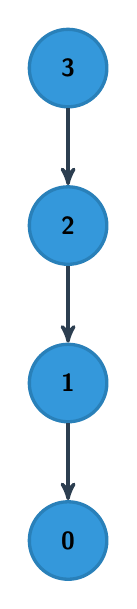
\begin{tikzpicture}[-,> = stealth',node distance=2.0cm, very thick]
    
      \node[commit] (0)              {0}[anchor=north];
      \node[commit] (1) [above of=0] {1};
      \node[commit] (2) [above of=1] {2};
      \node[commit] (3) [above of=2] {3};

      \path[arrow_commit]
        \foreach \y [count=\i] in {0,1,2} {
          (\y) edge node {} (\i)
        } ;
    \end{tikzpicture}
    
    \column{4.5cm}
      \fontHeadIV{
        \visible<2-4>{
          \tikz[na] \coordinate (commit);\cgray{Commit} \\
        }
        \visible<3-4>{
           \ \tikz[na] \coordinate (sha); \cgray{SHA1} \\
        }
      }
  \end{columns}
    
  % Brace with "Repository"
  \only<5>{
  \begin{tikzpicture}[overlay]
          \draw[decorate,decoration={brace,amplitude=12pt,mirror,raise=30pt},yshift=0pt,color=uigray,ultra thick]
               (0.south) -- (3.north) node [uigray,midway,xshift=4.5cm] {
                 \fontHeadIV{$Repository$}
               };
  \end{tikzpicture}
  }
  
  % Arrows overlay
  \begin{tikzpicture}[overlay]
    \path[<-,> = stealth',uigray,thick,transform canvas={xshift=-20pt}]<4->
      (3.west) edge node [uigray,xshift=-0.3cm,font=\Large]{t} (0.west);
    \path[<-,uigray,dashed,thick]<2-4>
      (2) edge node {} (commit);
    \path[<-,uigray,dashed,thick,shorten <= 3.8pt]<3-4>
      (1.center) edge [bend left=10] (sha);
  \end{tikzpicture}

\end{frame}

%-------------------------------------------------------------------
%                              Branches
%-------------------------------------------------------------------
%
\setbeamercolor{background canvas}{bg=uigreen_dark}
\section{Branches}
\begin{frame}
  \begin{center}
    \fontHeadII{\cred{Branches}}
  \end{center}
\end{frame}

\setbeamercolor{background canvas}{bg=uigreen}
\begin{frame}[c]
  \begin{center}
    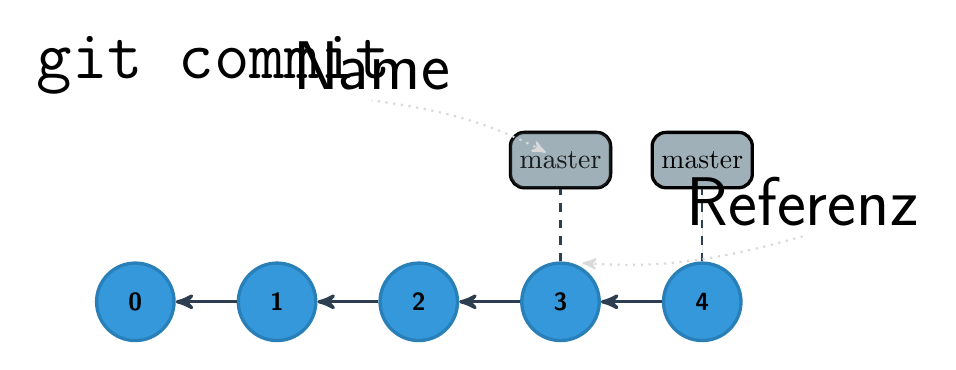
\begin{tikzpicture}[-,> = stealth',node distance=1.8cm, very thick]
      \node[commit] (0)              {0}[anchor=north];
      \node[commit] (1) [right of=0] {1};
      \node[commit] (2) [right of=1] {2};
      \node[commit] (3) [right of=2] {3};
      
      \visible<1-3>{
        \node[branch]  (master) [above of=3]  {master};
      }

      % Commit arrows
      \path[arrow_commit]
        \foreach \y [count=\i] in {0,1,2} {
          (\y) edge node {} (\i)
        } ;
        
      % Arrow branch to last commit
      \path[arrow_branch] (3) edge node [uigray,xshift=-0.3cm,font=\Large]{} (master);
      
      % Git commit
      \visible<4->{
        \node[commit] (4) [right of=3] {4};
        \path[arrow_commit] (3) -- (4);
        
        % Fade out old master
        \node[branch, opacity=0.2]  (master) [above of=3]  {master};
        
        % New master position
        \node[branch]  (master2) [above of=4]  {master};
        \path[arrow_branch] (4) -- (master2);
        
        % Git command
        \node[headline] (text_fetch) at (1,3) {\texttt{git commit}};
      }

      % "Name" string and arrow
      \visible<2-3>{
        \node[style={font=\sffamily\Huge}] (branch_name) at (3,3) {Name};
        \path[<-,uigray,dotted,thick,shorten <= 6.0pt]
          (master.center) edge [bend right=10] (branch_name.south);
      }
        
      % "Referenz" string and arrow
      \visible<3-3>{
        \node[style={font=\sffamily\Huge}] (branch_ref) [above right of=4] {Referenz};
        \path[<-,uigray,dotted,thick,shorten <= 8.0pt]
          (3.north) edge [bend right=10] (branch_ref.south);
      }

    \end{tikzpicture}
  \end{center}
\end{frame}

\setbeamercolor{background canvas}{bg=uigreen_dark}
\begin{frame}
  \begin{center}
    \fontHeadII{\cred{Mehrere}} \\ \vspace{1em}
    \fontHeadII{\cgray{Branches}}
  \end{center}
\end{frame}


\setbeamercolor{background canvas}{bg=uigreen}
\begin{frame}[c]
  \begin{center}
    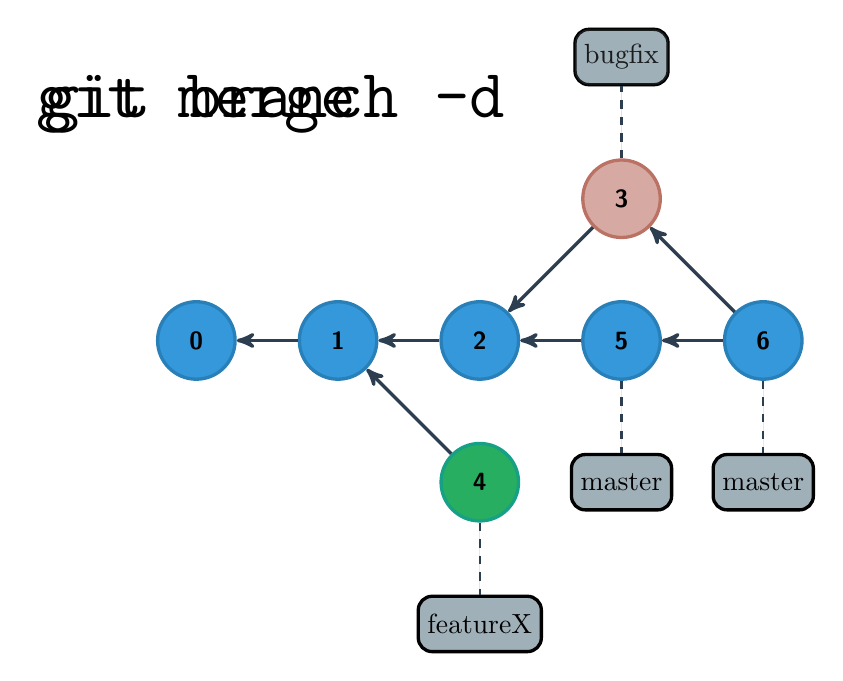
\begin{tikzpicture}[-,> = stealth',node distance=1.8cm, very thick]
      \node[commit] (0)              {0}[anchor=north];
      \node[commit] (1) [right of=0] {1};
      \node[commit] (2) [right of=1] {2};
      \node[commit] (5) [right of=2] {5};
      \node[commit2] (3) [above of=5] {3};
      \node[commit3] (4) [below of=2] {4};
      \node[branch] (featureX) [below of=4] {featureX};
      
      \visible<1-2>{
        \node[branch]  (bugfix) [above of=3]  {bugfix};
      }
      
      \visible<1>{
        \node[branch]  (master) [below of=5]  {master};
      }
      
      % Commit arrows
      \path[arrow_commit] (0) -- (1);
      \path[arrow_commit] (1) -- (2);
      \path[arrow_commit] (2) -- (5);
      \path[arrow_commit] (2) -- (3);
      \path[arrow_commit] (1) -- (4);
      
      \path[arrow_branch]<1> (5) -- (master);
      \path[arrow_branch]<1-2> (3) -- (bugfix);
      \path[arrow_branch] (4) -- (featureX);
      
      % More than one parent
      \visible<2->{
        \node[commit] (6) [right of=5] {6};
        \node[branch]  (master) [below of=6]  {master};

        \path[arrow_commit] (5) -- (6);      
        \path[arrow_commit] (3) -- (6);
        \path[arrow_branch] (6) -- (master);
      }
      
      \visible<2>{
        \node[headline] (text_merge) at (0,3) {\texttt{git merge}};
      }
      
      % Delete bugfix-Branch
      \visible<3->{
        \node[branch, opacity=0.2]  (bugfix) [above of=3]  {bugfix};
        \path[arrow_branch, opacity=0.2] (3) -- (bugfix);
        
        \node[headline] (text_delete) at (1,3) {\texttt{git branch -d}};
      }
    \end{tikzpicture}
  \end{center}
\end{frame}


%-------------------------------------------------------------------
%                                 HEAD
%-------------------------------------------------------------------
%
\setbeamercolor{background canvas}{bg=uigreen_dark}
\begin{frame}
  \begin{center}
    \fontHeadIII{\cred{Welcher Branch?}}
  \end{center}
\end{frame}

\setbeamercolor{background canvas}{bg=uigreen}
\begin{frame}[c]
  \begin{center}
    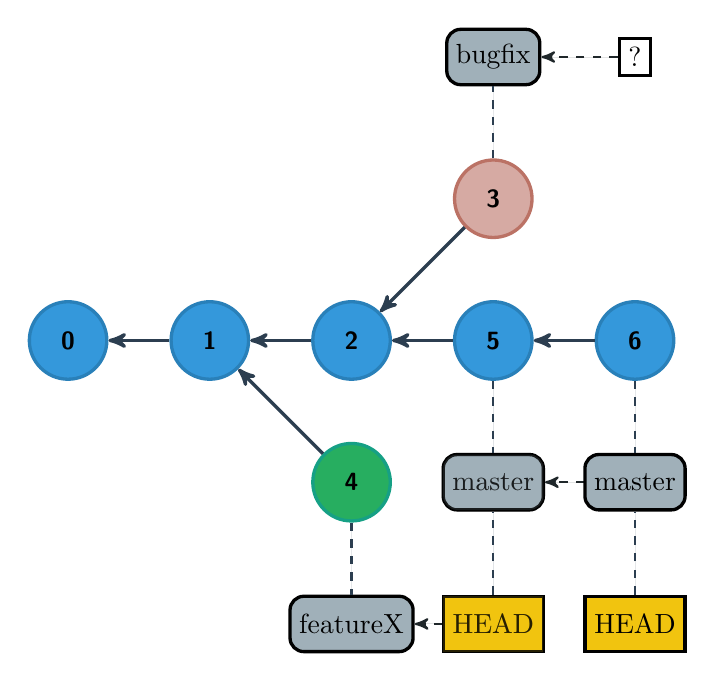
\begin{tikzpicture}[-,> = stealth',node distance=1.8cm, very thick]
      \node[commit] (0)              {0}[anchor=north];
      \node[commit] (1) [right of=0] {1};
      \node[commit] (2) [right of=1] {2};
      \node[commit] (5) [right of=2] {5};
      \node[commit2] (3) [above of=5] {3};
      \node[commit3] (4) [below of=2] {4};
      \node[branch] (featureX) [below of=4] {featureX};
      \node[branch]  (bugfix) [above of=3]  {bugfix};
      
      % Master branch
      \visible<1-3>{
        \node[branch]  (master) [below of=5]  {master};
        \path[arrow_branch] (5) -- (master);
      }
      
      % Commit arrows
      \path[arrow_commit] (0) -- (1);
      \path[arrow_commit] (1) -- (2);
      \path[arrow_commit] (2) -- (5);
      \path[arrow_commit] (2) -- (3);
      \path[arrow_commit] (1) -- (4);
      
      % Branch arrows
      \path[arrow_branch] (3) -- (bugfix);
      \path[arrow_branch] (4) -- (featureX);
      
      % Refs ?
      \visible<2>{
        \node[empty]  (head1) [right of=master]  {?};
        \node[empty]  (head2) [right of=bugfix]  {?};
        \node[empty]  (head3) [right of=featureX]  {?};
        
        \path[arrow_comment] (head1) -- (master);
        \path[arrow_comment] (head2) -- (bugfix);
        \path[arrow_comment] (head3) -- (featureX);
      }
      
      % Head ref
      \visible<3>{
        \node[head]  (head) [below of=master]  {HEAD};
        \path[arrow_head] (head) -- (master);
      }
      
      % Add commit
      \visible<4>{
        % Fade out old master/head
        \node[head, opacity=0.2]  (head) [below of=master]  {HEAD};
        \path[arrow_head, opacity=0.2] (head) -- (master);
        \node[branch, opacity=0.2]  (master) [below of=5]  {master};
        \path[arrow_branch, opacity=0.2] (5) -- (master);

        
        % Show new
        \node[commit] (6) [right of=5] {6};
        \path[arrow_commit] (5) -- (6);
        
        \node[branch]  (master) [below of=6]  {master};
        \path[arrow_branch] (6) -- (master);
        
        \node[head]  (head) [below of=master]  {HEAD};
        \path[arrow_head] (head) -- (master);
      }
      
    \end{tikzpicture}
  \end{center}
\end{frame}


%-------------------------------------------------------------------
%                                Tags
%-------------------------------------------------------------------
%
\setbeamercolor{background canvas}{bg=uigreen_dark}
\section{Tags}
\begin{frame}
  \begin{center}
    \fontHeadIII{\cred{Tags}}
  \end{center}
\end{frame}

\setbeamercolor{background canvas}{bg=uigreen}
\begin{frame}[c]
  \begin{center}
    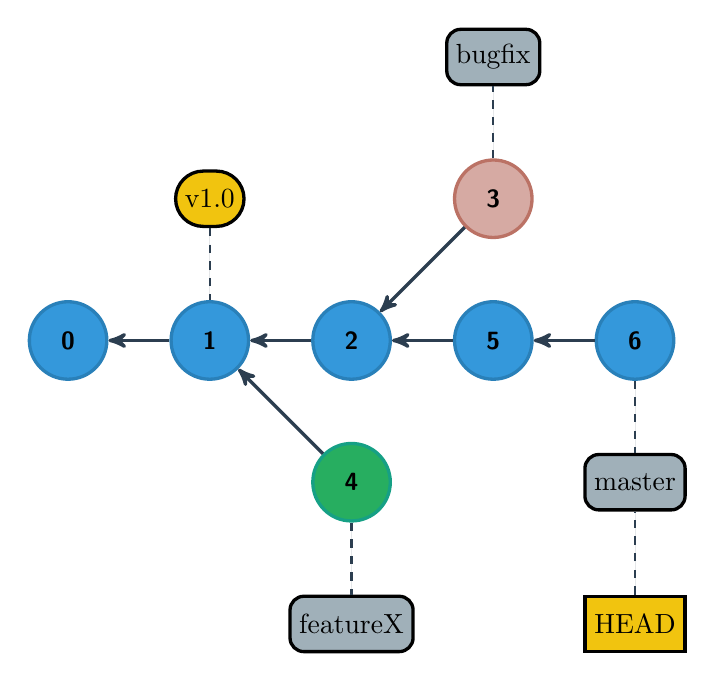
\begin{tikzpicture}[-,> = stealth',node distance=1.8cm, very thick]
      \node[commit] (0)              {0}[anchor=north];
      \node[commit] (1) [right of=0] {1};
      \node[commit] (2) [right of=1] {2};
      \node[commit] (5) [right of=2] {5};
      \node[commit2] (3) [above of=5] {3};
      \node[commit3] (4) [below of=2] {4};
      \node[commit] (6) [right of=5] {6};
      \node[branch]  (master) [below of=6]  {master};
      \node[branch] (featureX) [below of=4] {featureX};
      \node[branch]  (bugfix) [above of=3]  {bugfix};
      
      % Head
      \node[head]  (head) [below of=master]  {HEAD};
      \path[arrow_head] (head) -- (master);
      
      % Commit arrows
      \path[arrow_commit] (0) -- (1);
      \path[arrow_commit] (1) -- (2);
      \path[arrow_commit] (2) -- (5);
      \path[arrow_commit] (2) -- (3);
      \path[arrow_commit] (1) -- (4);
      \path[arrow_commit] (5) -- (6);

      % Branch arrows
      \path[arrow_branch] (6) -- (master);
      \path[arrow_branch] (3) -- (bugfix);
      \path[arrow_branch] (4) -- (featureX);
      
      % Tag
      \visible<2->{
        \node[tag] (tag1) [above of=1] {v1.0};
        \path[arrow_head] (tag1) -- (1);
      }

    \end{tikzpicture}
  \end{center}
\end{frame}

\setbeamercolor{background canvas}{bg=uigreen_dark}
\begin{frame}
  \begin{center}
    \setlength{\tabcolsep}{0pt}
    \begin{tabular}{r@{}l}
      \fontHeadIV{\cgreen{Branches}} & \fontHeadIV{\cgray{bewegen sich}} \\
      \fontHeadII{\cgreen{Tags}} & \fontHeadII{\cred{nicht!}} \\ 
    \end{tabular} 
  \end{center}
\end{frame}


%-------------------------------------------------------------------
%                                Remote
%-------------------------------------------------------------------
%
\setbeamercolor{background canvas}{bg=uigreen}
\section{Remote}
\begin{frame}
 \begin{center}
   \fontHeadI{\cdark{Remote}} \\
   \fontHeadIV{\cgray{Alias einer git-URL}} \\
  \end{center}
\end{frame}

\setbeamercolor{background canvas}{bg=uigreen}
\begin{frame}
  \begin{center}
    \vspace{-3.5em}
    \setlength{\tabcolsep}{0pt}
    \begin{tabular}{r@{}l}
      \fontHeadIV{\cdark{ssh}} &  \fontNormal{\cgray{ssh://[user@]host.xz[:port]/path/repo.git}} \\ 
      \fontHeadIV{\cdark{http}} & \fontNormal{\cgray{http[s]://host.xz[:port]/path/to/repo.git}} \\ 
      \fontHeadIV{\cdark{git}} &  \fontNormal{\cgray{git://host.xz[:port]/path/to/repo.git}} \\ 
      \fontHeadIV{\cdark{file}} & \fontNormal{\cgray{file:///full/path/to/reponame}} \\ 
    \end{tabular} 
  \end{center}
\end{frame}

\setbeamercolor{background canvas}{bg=uigreen_dark}
\begin{frame}
  \begin{center}
    \fontHeadII{\cred{Remote}} \\
    \vspace{2em}
    \fontHeadII{\cgray{Branches}}
  \end{center}
\end{frame}

\setbeamercolor{background canvas}{bg=uigreen}
\begin{frame}[c]
  \begin{center}
    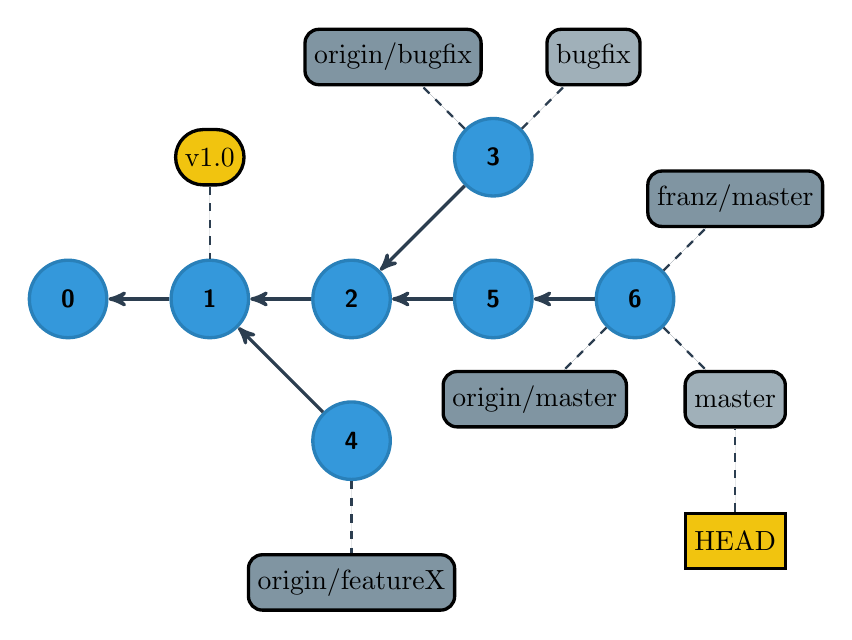
\begin{tikzpicture}[-,> = stealth',node distance=1.8cm, very thick]
      \node[commit] (0)              {0}[anchor=north];
      \node[commit] (1) [right of=0] {1};
      \node[commit] (2) [right of=1] {2};
      \node[commit] (5) [right of=2] {5};
      \node[commit] (3) [above of=5] {3};
      \node[commit] (4) [below of=2] {4};
      \node[commit] (6) [right of=5] {6};
      \node[branch]  (master) [below right of=6]  {master};
      \node[branch_remote]  (master_remote) [below left of=6]  {origin/master};
      \node[branch_remote] (featureX_remote) [below of=4] {origin/featureX};
      \node[branch] (bugfix) [above right of=3]  {bugfix};
      \node[branch_remote] (bugfix_remote) [above left of=3]  {origin/bugfix};
      
      % Head
      \node[head]  (head) [below of=master]  {HEAD};
      \path[arrow_head] (head) -- (master);
      
      % Commit arrows
      \path[arrow_commit] (0) -- (1);
      \path[arrow_commit] (1) -- (2);
      \path[arrow_commit] (2) -- (5);
      \path[arrow_commit] (2) -- (3);
      \path[arrow_commit] (1) -- (4);
      \path[arrow_commit] (5) -- (6);

      % Branch arrows
      \path[arrow_branch] (6) -- (master);
      \path[arrow_branch] (6) -- (master_remote);
      \path[arrow_branch] (3) -- (bugfix);
      \path[arrow_branch] (3) -- (bugfix_remote);
      \path[arrow_branch] (4) -- (featureX_remote);
      
      % Tag
      \node[tag] (tag1) [above of=1] {v1.0};
      \path[arrow_head] (tag1) -- (1);
      
      % Second remote master
      \visible<2->{
        \node[branch_remote]  (master_remote2) [above right of=6]  {franz/master};
        \path[arrow_branch] (6) -- (master_remote2);
      }

    \end{tikzpicture}
  \end{center}
\end{frame}

%-------------------------------------------------------------------
%                                Fetch
%-------------------------------------------------------------------
%
\setbeamercolor{background canvas}{bg=uigreen_dark}
\section{Fetch}
\begin{frame}
  \begin{center}
    \fontHeadII{\cred{Fetch}} \\
  \end{center}
\end{frame}


% Hier besonders darauf hinweisen, dass sich der sha-Wert nach dem mergen nicht aengert!
% Blobs/commits ist es egal wo sie herkommen.
\setbeamercolor{background canvas}{bg=uigreen}
\begin{frame}[c]
  \begin{center}
    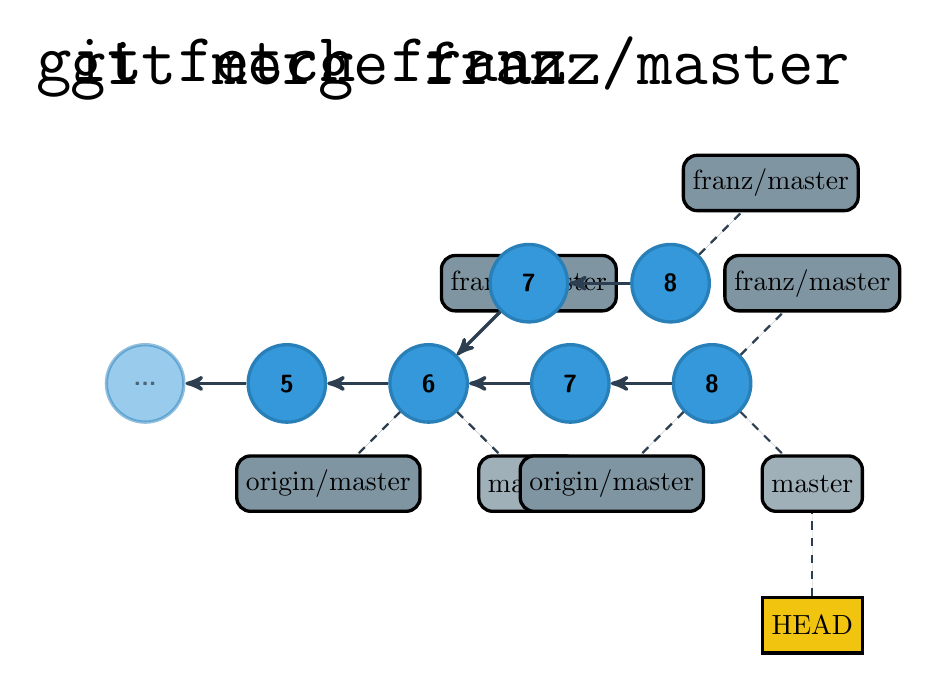
\begin{tikzpicture}[-,> = stealth',node distance=1.8cm, very thick]
      \node[commit, opacity=0.5] (etc) at (0, 2)  {...};
      \node[commit] (5) [right of=etc] {5};
      \node[commit] (6) [right of=5] {6};
      
      % Commit arrows
      \path[arrow_commit] (etc) -- (5);
      \path[arrow_commit] (5) -- (6);

      \visible<1>{
        % Remote branch franz
        \node[branch_remote]  (master_remote2) [above right of=6]  {franz/master};
        \path[arrow_branch] (6) -- (master_remote2);
      }
      
      \visible<1-2>{
        % Master
        \node[branch]  (master) [below right of=6]  {master};
        \node[branch_remote]  (master_remote) [below left of=6]  {origin/master};
        
        % Branch arrows
        \path[arrow_branch] (6) -- (master);
        \path[arrow_branch] (6) -- (master_remote);
        

      }
      
      % Commits from franz
      \visible<2>{
        \node[commit] (7) [above right of=6] {7};
        \node[commit] (8) [right of=7] {8};
        \path[arrow_commit] (6) -- (7);
        \path[arrow_commit] (7) -- (8);
        
        \node[branch_remote]  (master_remote2) [above right of=8]  {franz/master};
        \path[arrow_branch] (8) -- (master_remote2);
        
        \node[headline,align=left] (text_fetch) at (2,6) {\texttt{git fetch franz}};
      }
      
      \visible<3>{
        \node[commit] (7) [right of=6] {7};
        \node[commit] (8) [right of=7] {8};
        \path[arrow_commit] (6) -- (7);
        \path[arrow_commit] (7) -- (8);
        
        % Master
        \node[branch]  (master) [below right of=8]  {master};
        \node[branch_remote]  (master_remote) [below left of=8]  {origin/master};
        
        % Branch arrows
        \path[arrow_branch] (8) -- (master);
        \path[arrow_branch] (8) -- (master_remote);
        
        % Head
        \node[head]  (head) [below of=master]  {HEAD};
        \path[arrow_head] (head) -- (master);
        
        % Remote franz
        \node[branch_remote]  (master_remote2) [above right of=8]  {franz/master};
        \path[arrow_branch] (8) -- (master_remote2);
        
        % Git command
        \node[headline] (text_fetch) at (4,6) {\texttt{git merge franz/master}};
      }
    \end{tikzpicture}
  \end{center}
\end{frame}

%-------------------------------------------------------------------
%                                 Merge
%-------------------------------------------------------------------
%
\setbeamercolor{background canvas}{bg=uigreen_dark}
\section{Merge}
\begin{frame}
  \begin{center}
    \fontHeadII{\cred{Merge}} \\
  \end{center}
\end{frame}

\setbeamercolor{background canvas}{bg=uigreen}
\begin{frame}[c]
  \begin{center}
    \begin{tikzpicture}[-,> = stealth',node distance=1.8cm, very thick]
      \node[commit, opacity=0.5] (etc) at (0, 2)  {...};
      \node[commit] (6) [right of=etc] {6};
      
      % Commit arrows
      \path[arrow_commit] (etc) -- (6);
      
      % Remote branch
      \node[branch_remote]  (master_remote) [below left of=6]  {origin/master};
      \path[arrow_branch] (6) -- (master_remote);

      \visible<1>{
      % Master
        \node[branch]  (master) [below right of=6]  {master};
        \path[arrow_branch] (6) -- (master);

        % Head
        \node[head]  (head) [below of=master]  {HEAD};
        \path[arrow_head] (head) -- (master);
      }
      
      % Add two more local commits
      \visible<2->{
        \node[commit] (9) [right of=6] {9};
        \node[commit] (10) [right of=9] {10};
        
        % Commit arrows
        \path[arrow_commit] (6) -- (9);
        \path[arrow_commit] (9) -- (10);
      }
      
      % New master position after two commits
      \visible<2>{
        \node[branch]  (master) [below right of=10]  {master};
        \path[arrow_branch] (10) -- (master);
        
        % Head
        \node[head]  (head) [below of=master]  {HEAD};
        \path[arrow_head] (head) -- (master);
        
        % Git commit command
        \node[headline] (text_commit) at (1,6) {\texttt{git commit}};
      }
      
      % After merge
      \visible<3->{
        \node[commit] (11) [right of=10] {11};
        \path[arrow_commit] (10) -- (11);
        \path[arrow_commit] (8) -- (11);
      }
      
      % New master position after merge
      \visible<3>{
        \node[branch]  (master) [below right of=11]  {master};
        \path[arrow_branch] (11) -- (master);
        
        % Head
        \node[head]  (head) [below of=master]  {HEAD};
        \path[arrow_head] (head) -- (master);
        
        % Git merge command
        \node[headline] (text_merge) at (1,6) {\texttt{git merge}};
      }

      % Commits from franz
      \node[commit3] (7) [above of=9] {7};
      \node[commit3] (8) [right of=7] {8};
      \path[arrow_commit] (6) -- (7);
      \path[arrow_commit] (7) -- (8);

      \node[branch_remote]  (master_remote2) [above right of=8]  {franz/master};
      \path[arrow_branch] (8) -- (master_remote2);

    \end{tikzpicture}
  \end{center}
\end{frame}

\end{document}
